% !TeX program = lualatex
% !TeX spellcheck = en_GB
\documentclass[a4paper,10pt]{article}

\usepackage{array}
\usepackage[%
    style=authoryear,
    isbn=false,
    url=false,
]{biblatex}
\usepackage{enumitem}
\usepackage{etoolbox}
\usepackage{float}
\usepackage{fontspec}
\usepackage[margin=0.5in]{geometry}
\usepackage{graphicx}
\usepackage{lua-ul} % underline for lualatex
%\usepackage{soul} % for underlines, doesn't work with superscript
\usepackage{tabularray}
\UseTblrLibrary{booktabs}
\usepackage{textcomp}
\usepackage{titlesec}
\usepackage{xcolor}
\usepackage{xparse}
\usepackage{hyperref}


% Settings
\hypersetup{%
    colorlinks,
    urlcolor=magenta5,
}
\titleformat{\section} % command
    [display] % shape
    {\Large\sectionfont\color{sectioncolor}} % format
    {} % label
    {0em} % sep
    {} % before-code
    [\vspace{-0.8em}\rule{\textwidth}{0.7pt}] % after-code
\titlespacing*{\section}{0em}{-1.5em}{0em}
\setlist[itemize]{
    % vertical spacing
    topsep=0em,
    itemsep=0em,
    % horizontal spacing
    %labelindent=0em,
    leftmargin=1em,
    labelsep=*,
}
\setlist[enumerate]{
    % vertical spacing
    topsep=0em,
    itemsep=0em,
    % horizontal spacing
    %labelindent=0em,
    leftmargin=1em,
    labelsep=*,
}
\setmainfont{Cabin}
\newfontfamily{\arvo}{Arvo}
\newfontfamily{\clearSans}{Clear Sans}
\def\sectionfont{\clearSans}
\def\projectfont{\arvo}
\definecolor{projectcolor}{HTML}{003865}
\definecolor{sectioncolor}{HTML}{EF5B0C}
\definecolor{infocolor}{HTML}{000000}
\SetTblrStyle{foot}{font=\footnotesize\vspace{-0.5em}}



% openfoam related
\newcommand{\of}{\href{https://openfoam.org/}{\texttt{OpenFOAM}}}
\newcommand{\rcf}{\texttt{rhoCentralFoam}}
\newcommand{\rcfrk}{\texttt{rhoCentralFoamRK3}}
\newcommand{\apupfrk}{\texttt{ausmPlusUpFoamRK3}}
\newcommand{\apup}{AUSM\textsuperscript{+}-up}
% other softwares
\newcommand{\feap}{\href{https://www.cs.cornell.edu/~bindel//blurbs/feap.html}{\texttt{FEAP}}}
% other commands
\newcommand{\duration}[1]{\hfill[#1]}
\ExplSyntaxOn
\NewDocumentCommand{\highlight}{%
    O{1} % highlighting level
    m % the word to highlight
}{%
    \int_case:nnF{#1}{%
        {1}{\textbf{#2}} % highlight level 1
        {2}{\underLine{#2}} % level 2
        {3}{\emph{#2}} % level 3
    }
    {#2} % default
}
\ExplSyntaxOff
\NewDocumentCommand{\project}{% prints out project details
    m % project name/title
    m % project supervisor
    m % venue
    m % duration
}{%
    {%
        \color{projectcolor}
        {\projectfont#1}\duration{#4}\\%
        {#2 $\vert$ #3}
    }
}



\addbibresource{../publications/publications.bib}



\begin{document}
\setlength{\intextsep}{0.1em}
\setlength{\textfloatsep}{0.1em}
\pagenumbering{gobble}
{
    \noindent\color{infocolor}
    \begin{minipage}{0.07\textwidth}
        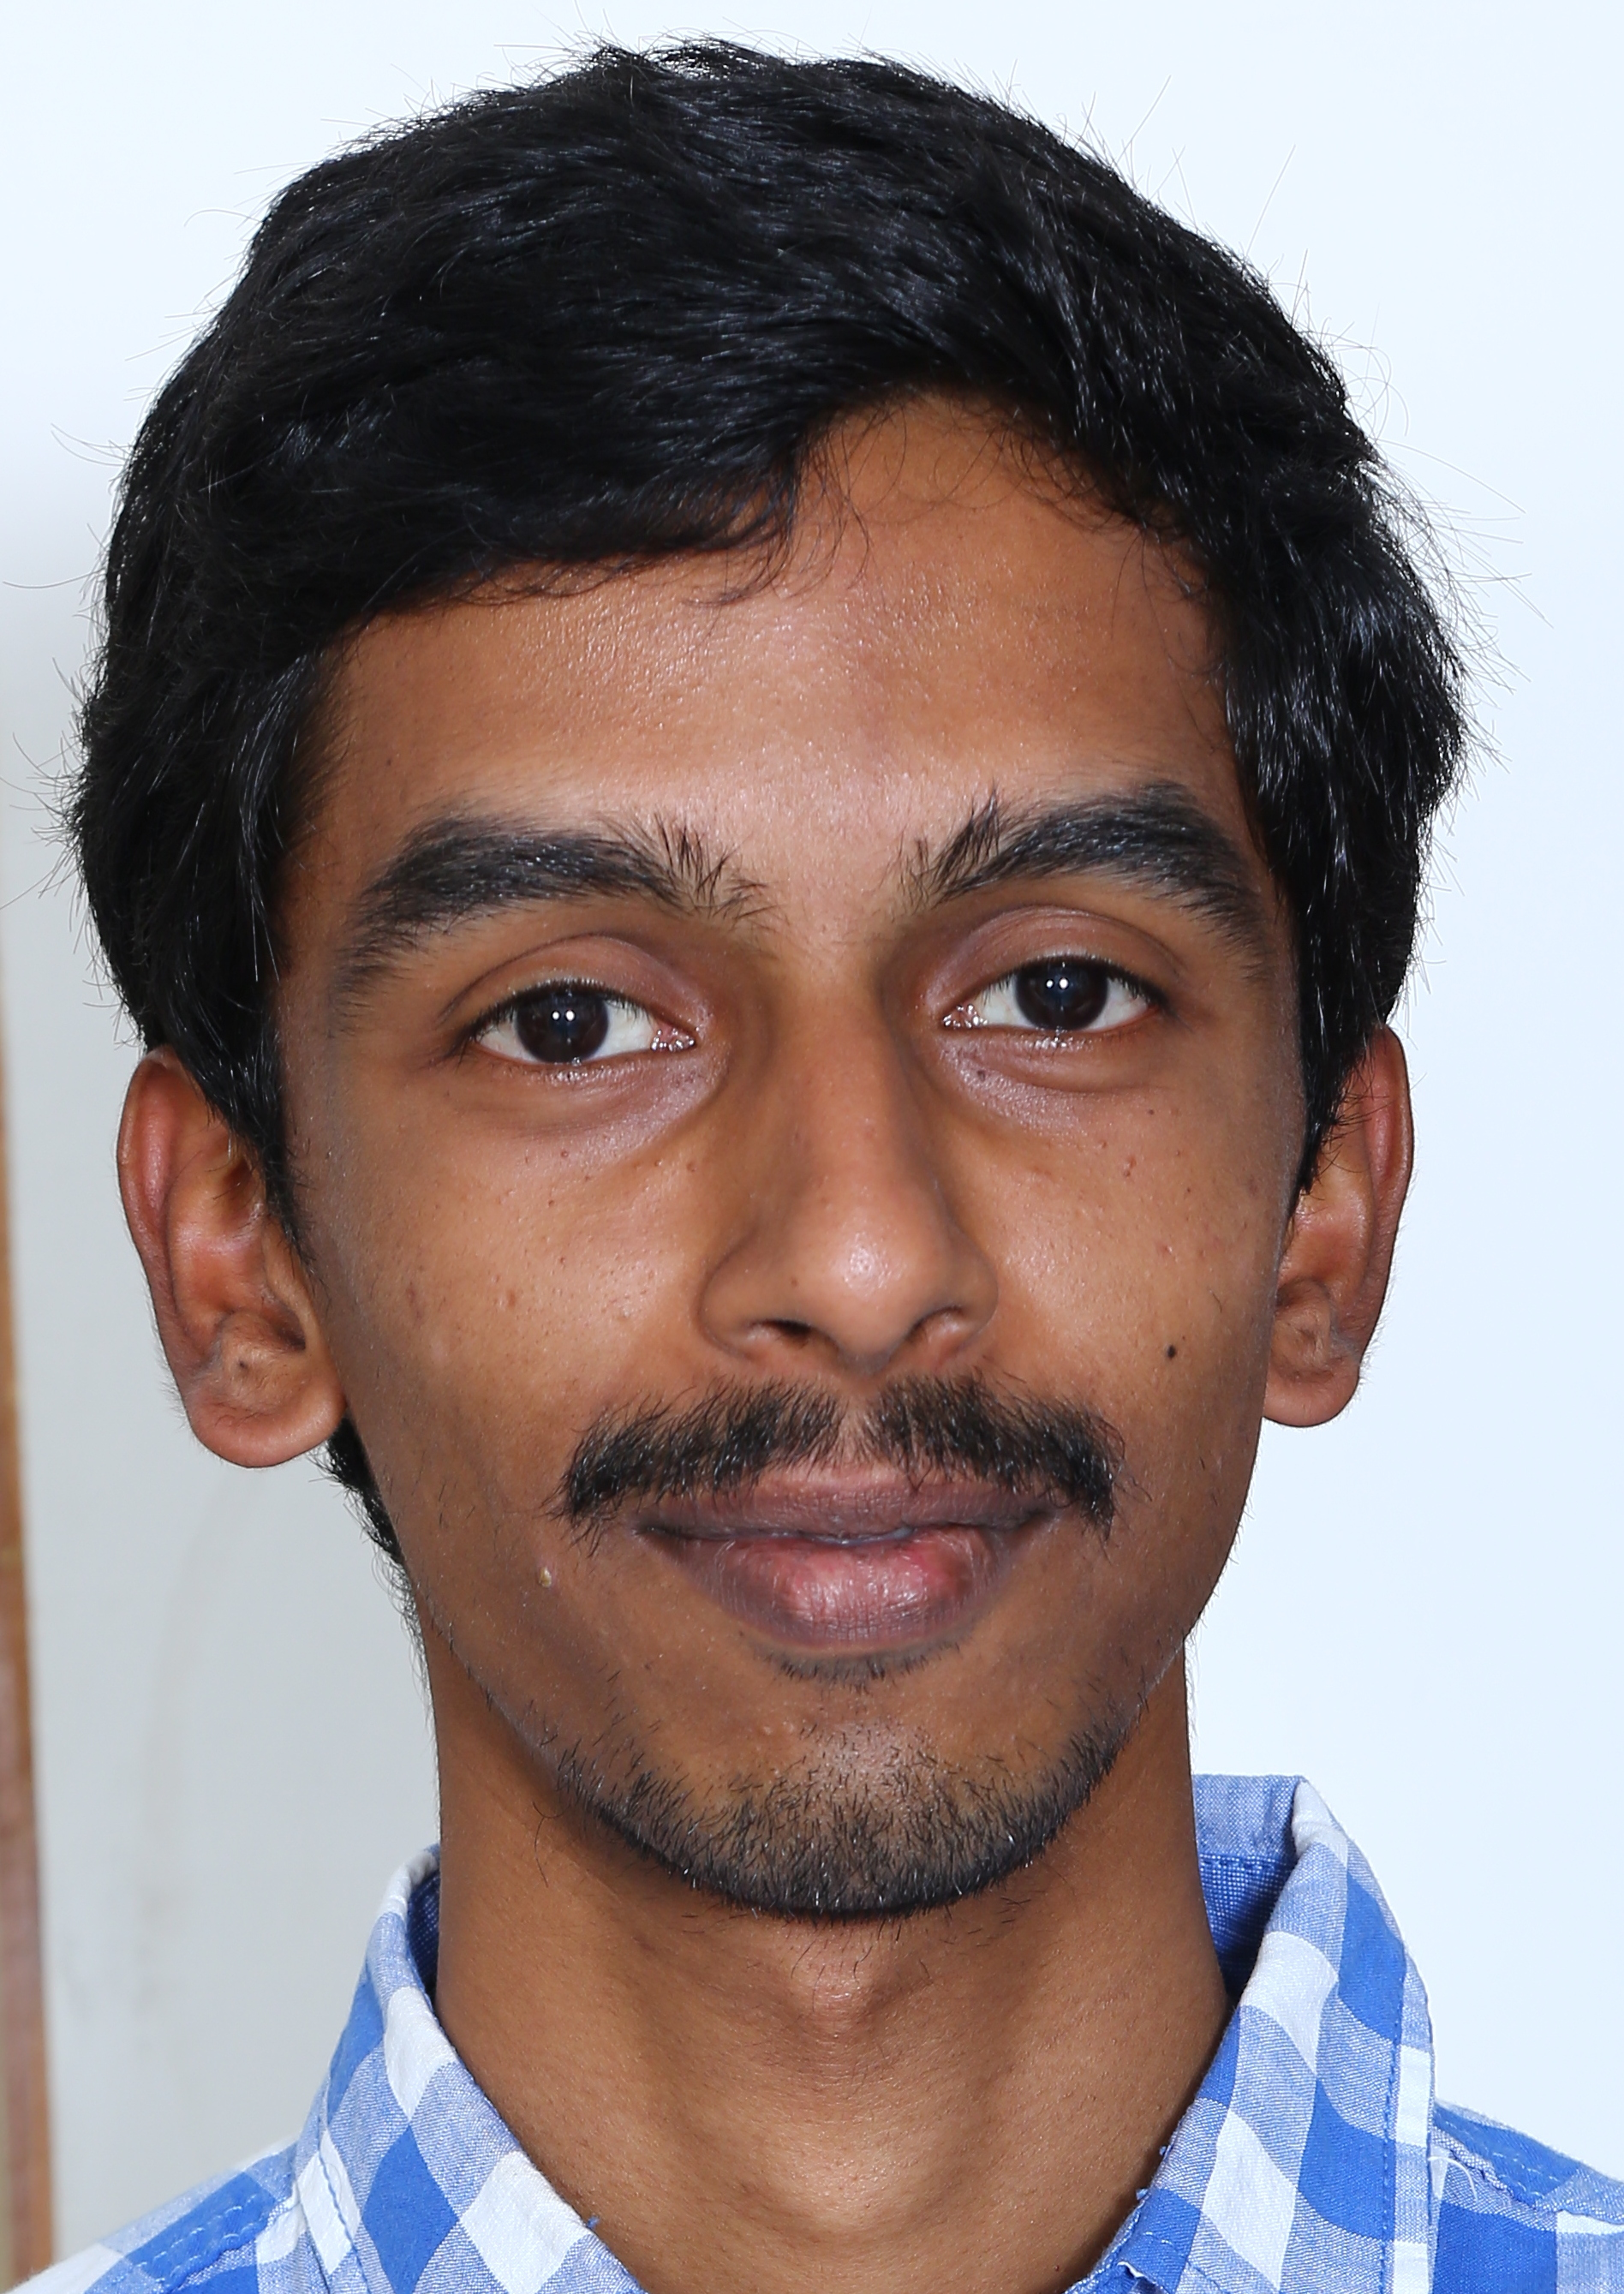
\includegraphics[width=\linewidth]{photo}
    \end{minipage}%
    \hspace{1em}
    \begin{minipage}{0.5\textwidth}
    	Potluri Vachan Deep\\
        Male\\
        DOB: 24-01-1997\\
        \url{https://vachan-potluri.github.io/}
    \end{minipage}%
    \hfill
    \begin{minipage}{0.4\textwidth}
    	\flushright
    	Ph.D. research scholar\\
        Mechanical Engineering Department\\
        Indian Institute of Technology Bombay
    \end{minipage}\\
}
%%%%
\begin{table}[H]
    \centering
    \begin{talltblr}[%
        label={none},
        note{*}={Expected year of completion},
    ]{%
        colspec={X[-3] X[-5] X[-5] X[-2] X[-1]},
        row{even}={gray!10},
        row{3,4}={m},
        row{1}={cmd=\bfseries},
    }
       	\toprule
        Examination & University & Institute & Year & CPI/\%\\
        \midrule
        Ph.D. & IIT Bombay & IIT Bombay & 2023\TblrNote{*} & 9.86 \\
        B.Tech. & IIT Bombay & IIT Bombay & 2018 & 9.72 \\
        Intermediate/+2 & Andhra Pradesh Board of Intermediate Education & Excel Junior College & 2014 & 97.3\\
        Matriculation & Andhra Pradesh Board of Secondary Education & Vardhana School & 2012 & 9.70\\
        \bottomrule
    \end{talltblr}
\end{table}
%%%%
\section{Publications}
\nocite{potluriPuranikBodi2022,potluriPuranikBodi2023}
\printbibliography[%
    heading=none,
]
%%%%
\section{Projects}
\begin{itemize}
	\item \project{Development of high resolution schemes for compressible flows in \of}%
		{Prof. Bhalchandra Puranik}%
		{Mechanical Engineering Department, IIT Bombay}%
		{Dec `16 -- Apr `18}
	\begin{itemize}
		\item \highlight{Modified an existing solver} \rcf{} to use \highlight[2]{TVD-RK3 time integration} scheme
		\item \highlight{Developed a new solver} \apupfrk{} that uses \highlight[2]{\apup{} flux scheme} along with RK3 time integration scheme
		\item \highlight{Performed a comparative study} using these two solvers by conducting simulations of several 1D and 2D test cases to draw useful conclusions
	\end{itemize}
	\item \project{Unified 2D Finite Element}
		{Prof. Parag Tandiya}
		{Mechanical Engineering Department, IIT Bombay}
		{Mar `18 -- Apr `18}
	\begin{itemize}
		\item \highlight{Implemented a subroutine} in FORTRAN77 library \feap{} for a \highlight[3]{new combined Plane Stress, Plain Strain and Axi--symmetric linear elasto--static element}, and validated the subroutine using several simple test cases
	\end{itemize}
	\item \project{Stair climbing wheel chair}
		{Prof. Shantanu Tripathi}
		{Mechanical Engineering Department, IIT Bombay}
		{Jun `17 -- Dec `17}
	\begin{itemize}
		\item \highlight{Proposed a mechanism} for a \highlight[2]{passive wheel chair} capable of \highlight[2]{climbing stairs} using the \highlight[3]{force provided by a companion}
		\item \highlight{Built} a \highlight[2]{full scale basic functioning prototype} \highlight[3]{within 2 months} constraining to the alloted budget and resources
		\item \highlight{Tested the prototype} on 2 different stair geometries and demonstrated it's effectiveness to Mechanical Engineering Department faculty, staff, and other students
	\end{itemize}
%	\item \projecttitle{Rarified Gas Flows}
%		{Prof. Amit Agrawal}
%		{Mechanical Engineering Department, IIT Bombay}
%		{May `16 -- June `16}
%		{Verifying simulations of flows in continuum--transition regime with Augmented Burnett equations}
%	\begin{itemize}[leftmargin=*]
%		\item Written a finite difference based MATLAB code to verify 2D experimental/simulation data with Augmented Burnett equations and validated it with Navier--Stokes solution
%		\item Tested the code with Monte Carlo type Direct Simulation data of 0.01 Knudsen Number flow and obtained normalized error of order 10\%\
%	\end{itemize}
\end{itemize}
%%%%
\section{Internships}
\begin{itemize}
	\item \project{GE90 HPC airfoil durability analysis}
	{Mr. Nageswara Ganji, Mr. Devesh Ojha}
	{John F. Welch Technology Center, General Electric}
	{May `17 -- Jul `17}
	\begin{itemize}
		\item \highlight{Modified} the \highlight[2]{mesh} of existing GE90-115B high pressure compressor stage-9 rotor blade, to model
		\begin{enumerate}
			\item Three types of \highlight[2]{damaged blades} by \highlight[3]{making notches} at different locations on the leading edge
			\item A \highlight[2]{defectively manufactured blade} by \highlight[3]{changing thickness of leading edge} according to manufacturing tolerance
		\end{enumerate}
		\item \highlight{Generated Campbell Diagrams} by \highlight[2]{simulating the vibration response} and \highlight{recalculated fatigue factor of safety}\ at critical locations of undamaged, damaged and defected blades for \highlight[2]{3 different materials}
	\end{itemize}
\end{itemize}
%%%%
\section{Scholastic Achievements}
\begin{itemize}
	\item \highlight{Stood 2nd in Department} out of more than \highlight[2]{150 students} in B.Tech. \duration{May `18}
	\item \highlight{Scored 829} in \highlight[2]{Graduate Aptitude Test in Engineering (GATE) 2018} \duration{Mar `18}
	\item \highlight{Secured All India Rank 129} in \highlight[2]{JEE Advanced 2014} in general category \duration{May `14}
	\item Awarded \highlight{Kishore Vigyanik Protshahan Yogana} (KVPY) fellowship by Indian Institute of Science (IISc), Bangalore \duration{Dec `13}
	\item \highlight{Secured position among top 1\%\ students} of former Andhra Pradesh who participated in \highlight[2]{National Standard Examination in Physics (NSEP)} \duration{Dec `13}
\end{itemize}
\end{document}